
\documentclass{report}

\usepackage[utf8]{inputenc}
\usepackage[italian]{babel}
\usepackage{import}
\usepackage{todonotes}
\usepackage{color}
\usepackage{rotating}
\usepackage[hidelinks]{hyperref}
\usepackage{url}
\usepackage{pdfpages}
\usepackage{siunitx}
\usepackage{pdflscape}
\usepackage{subfig}
\usepackage[euler]{textgreek}
\usepackage{mhchem}

\usepackage{multirow}

\usepackage{enumerate} 
\usepackage{amsmath}
\usepackage{amsfonts}

\usepackage[signatures,swapnames,sans]{frontespizio}

\usepackage{geometry}
\geometry{portrait, margin=3cm}
\usepackage{siunitx}
\usepackage{booktabs}

\renewcommand*\figurename{Figura}

\newcommand{\sub}[1]{\textsubscript{#1}}
\newcommand{\super}[1]{\textsuperscript{#1}}
\newcommand{\parallelsum}{\mathbin{\!/\mkern-5mu/\!}}

\newcommand{\Fig}[0]{Fig.}

\usepackage{titlesec}

\titleformat{\chapter}{\normalfont\huge}{}{20pt}{\huge\bfseries}

\linespread{1.3}


%% COMANDI UTILI
%\begin{table}[h]
%	\centering
%	\begin{tabular}{|c|c|c|}
%	\cline{2-3} 
%	\multicolumn{1}{c|}{} & \textbf{Valore nominale} & \textbf{Valore misurato}\\ 
%		%\hline
%		%{} & \textbf{Valore nominale} & \textbf{Valore misurato} \\ 
%		\hline
%		$\mathbf{R_1}$ & \SI{18}{k\ohm} & \SI{17.977}{k\ohm} \\ 
%		\hline
%		$\mathbf{R_2}$& \SI{1.8}{k\ohm} & \SI{1.815}{k\ohm} \\ 
%		\hline
%	\end{tabular}
%\caption{Misure delle resistenze utilizzate per il circuito.}
%\label{table:mis_res}
%\end{table}
%\begin{figure}[h!]
%\centering
%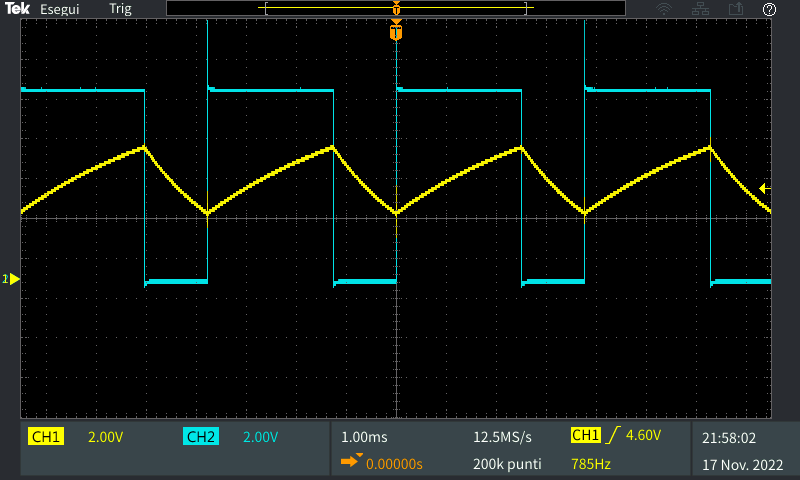
\includegraphics[height=6.5cm]{immagini/TEK00018}\\(a)\\[1ex]
%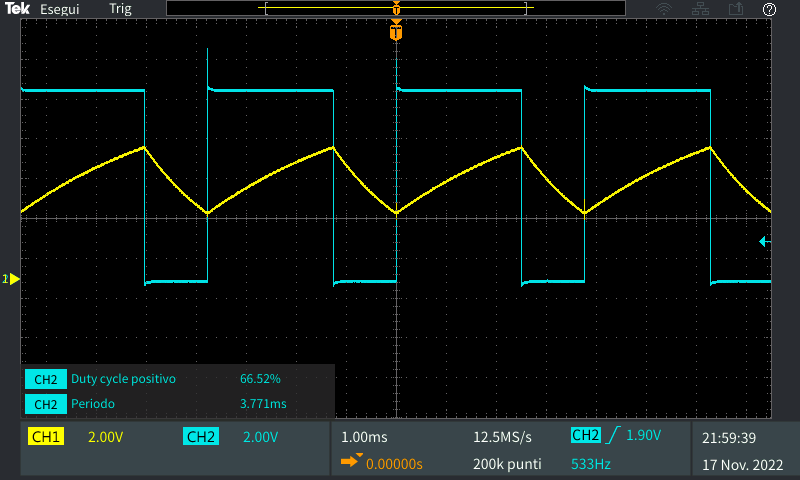
\includegraphics[height=6.5cm]{immagini/TEK00019}\\(b)
%\caption{Risposta del circuito con accoppiamento DC (a) e accoppiamento AC (b).}
%	\label{figura:accopp}
%\end{figure}

\begin{document}
\addtocounter{chapter}{+4}
	\begin{frontespizio}
		\Margini{3cm}{3cm}{3cm}{3cm}
		\Universita{Bergamo}
		\Logo[43.332mm]{unibg-mark}
		\Divisione{Scuola di Ingegneria}
		\Corso[Laurea Magistrale]{Ingegneria Informatica}
		\Titolo{Laboratorio di Elettronica}
		\Sottotitolo{Relazione esperienza di laboratorio 5}
		\Punteggiatura{}
		\NRelatore{Prof.}{Prof.}
		\Relatore{Luigi Gaioni}
		\Candidato[1058231]{Giulia Allievi}
		\Candidato[1059640]{Martina Fanton}
		\Annoaccademico{2022--2023}
		\begin{Preambolo*}
			\usepackage[italian]{babel}
			\usepackage[T1]{fontenc}
			\usepackage[utf8]{inputenc}
			\usepackage{microtype}
			\usepackage{lmodern}
			\graphicspath{{img/}}
			
			\renewcommand{\frontinstitutionfont}{\fontsize{14}{17}\bfseries\scshape}
			\renewcommand{\fronttitlefont}{\fontsize{17}{21}\bfseries\scshape}
			\renewcommand{\frontfootfont}{\fontsize{12}{14}\bfseries\scshape}
		\end{Preambolo*}
	\end{frontespizio}

%----------------------------------------------------------------------------------------
%	PAGINA BIANCA
%----------------------------------------------------------------------------------------
\newpage
\null
\thispagestyle{empty}
\newpage

%----------------------------------------------------------------------------------------
%	INTRO
%----------------------------------------------------------------------------------------
\chapter{Relazione attività di laboratorio 5}
\section*{Introduzione}
In quest'attività di laboratorio abbiamo visto un ultimo circuito monostabile con LM555, successivamente sono state analizzate le altre due configurazioni realizzabili con questo circuito integrato (prima la configurazione bistabile e dopo quella astabile).  \par
La seconda modalità, quella astabile, permette di generare in uscita al pin 3 un'onda quadra le cui caratteristiche dipendono dalla rete collegata all'esterno del circuito integrato. Le connessioni sono illustrate nel datasheet del componente, si riporta di seguito lo schema (figura \ref{figura:datasheet1}).
\begin{figure}[h!]
	\centering
	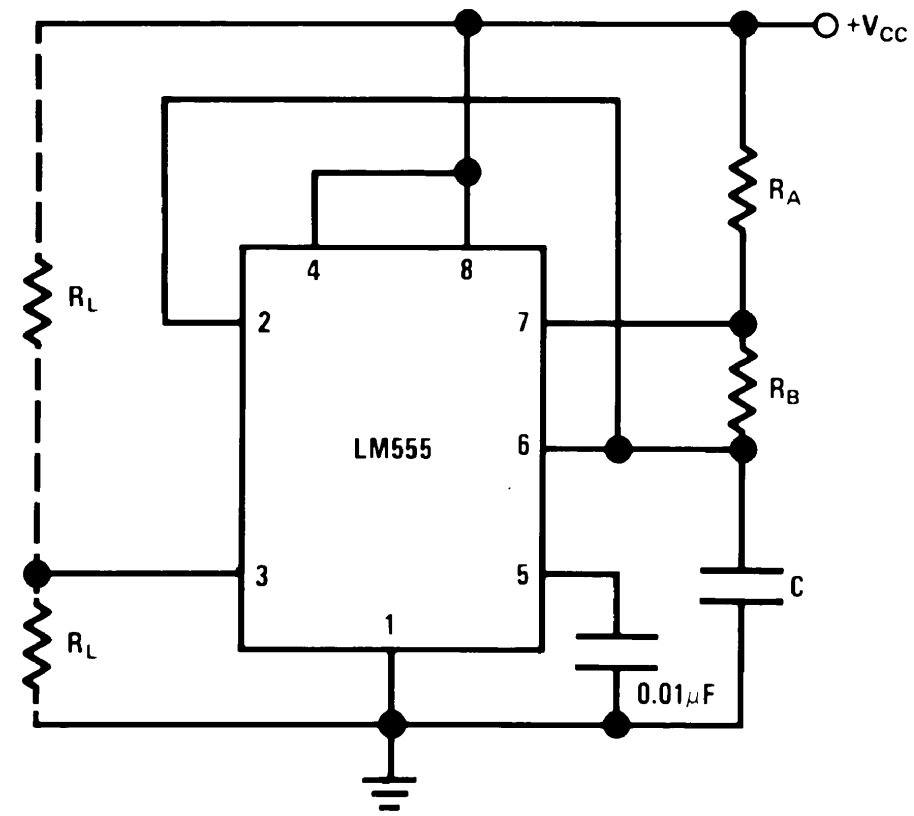
\includegraphics[height=6cm]{immagini/datasheet1}
	\caption{Schema delle connessioni da utilizzare per ottenere un circuito astabile (fonte: \textcolor{blue}{\underline{\href{https://www.ti.com/lit/ds/symlink/lm555.pdf?ts=1667144089940&ref_url=https\%253A\%252F\%252Fwww.ti.com\%252Fproduct\%252FLM555}{datasheet}}}).} % LM o NE ??
	\label{figura:datasheet1}
\end{figure}
\\ La configurazione bistabile invece non è presentata nel datasheet. Questa modalità è utile quando si vuole utilizzare il LM555 come flip-flop set reset. Per ottenerla, è sufficiente utilizzare due resistenze e due pulsanti. Una resistenza è collegata tra i pin 8 e 2, l'altra invece è collegata tra i pin 4 e 8; per quanto riguarda i due pulsanti, uno è collegato tra i pin 2 e 1 e pilota il set, mentre l'altro è connesso ai pin 4 e 1 e comanda il reset. Il pin 8 è collegato all'alimentazione, il pin 1 a massa, il segnale è prelevato al pin 3 e tutti gli altri pin sono lasciati floating. Lo schema si trova nella sezione dedicata all'analisi di questo circuito (sezione \ref{sez2}, figura \ref{figura:schema2}).

\newpage
\section{Circuito 1: LM555 in configurazione monostabile con switch debouncing}
\subsection{Schema del circuito e Funzione di Trasferimento}
Questo circuito è basato sull'ultimo circuito analizzato nello scorso laboratorio (ovvero il circuito monostabile con LM555). La differenza più evidente tra i due circuiti è rappresentata dal fatto che il circuito in esame riceve in ingresso un segnale di trigger generato da un pulsante, mentre il precedente circuito riceveva in ingresso un segnale di trigger fornito da un generatore di forme d'onda.

Questo circuito, mostrato in figura \ref{figura:schema1}, presenta: due resistenze (R è collegata tra il pin 7 e l'alimentazione positiva, mentre $\mathrm{R_1}$ tra il pin 2 e l'alimentazione positiva), due capacità ($\mathrm{C_1}$ è collegata tra il pin 6 e la massa, mentre $\mathrm{C_2}$ tra il pin 5 e la massa) e un pulsante collegato tra il pin 2 e la massa.

\begin{figure}[h!]
	\centering
	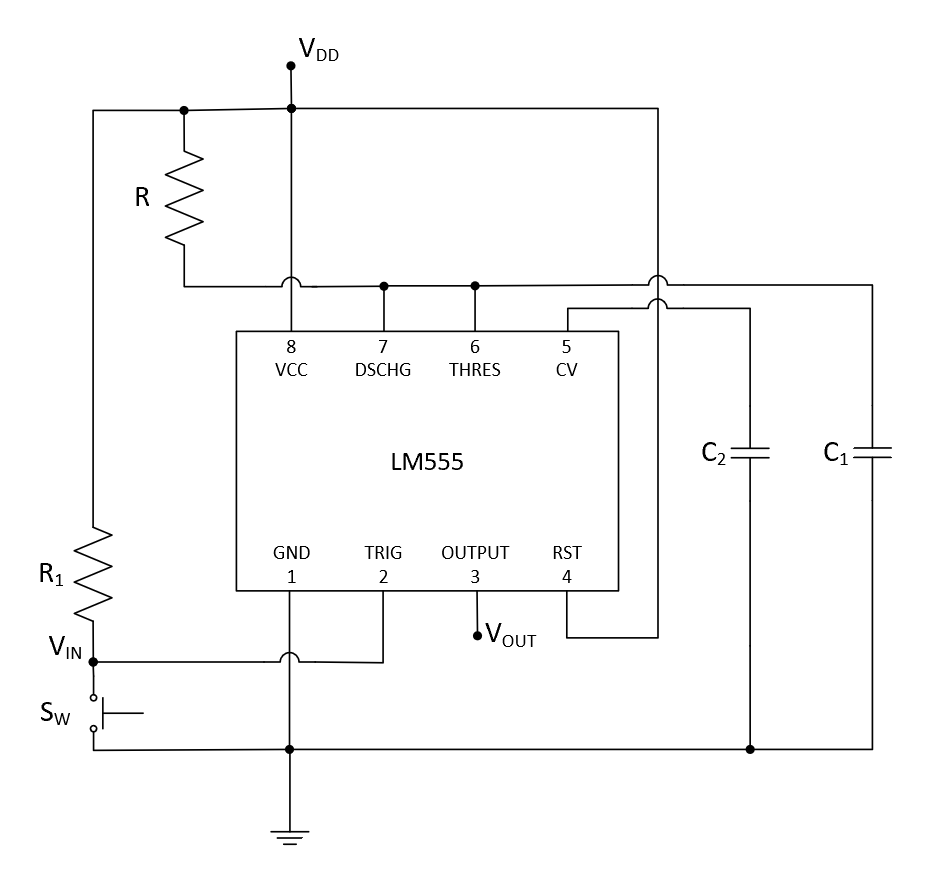
\includegraphics[height=7.5cm]{immagini/schema1}
	\caption{Schema del circuito monostabile con switch debouncing.}
	\label{figura:schema1}
\end{figure}

\noindent La caratteristica principale di questo circuito consiste nel correggere l'effetto del rimbalzo dell'interruttore (\textit{switch debouncing}, visibile nella figura \ref{figura:TEK00009}). Questo effetto, che consiste nella generazione di un treno di impulsi spuri su entrambi i fronti dell'impulso in ingresso, viene prodotto soltanto dalla rete antecedente il timer e in particolare è dovuto al fatto che la chiusura e l'apertura del pulsante non avvengono in modo istantaneo. Quindi l'aggiunta del LM555 alla rete in ingresso determina un segnale in uscita filtrato da questo effetto indesiderato poichè il timer genera un solo impulso in uscita non appena riceve il primo fronte di discesa del segnale in ingresso.

La funzione di trasferimento di questo circuito è:
\begin{equation}
	\begin{cases}
		V_{out}= V_{DD}\indent\indent \mathrm{a\;partire\;dalla\;chiusura\;di\;} S_W \mathrm{\;e\;per\;una\;durata\;T\;}\\[5pt]
		V_{out}= 0\indent\indent\indent \mathrm{altrimenti}\\
	\end{cases}
\end{equation}

\subsection{Analisi e dati sperimentali}
Per quanto riguarda la scelta e il dimensionamento dei componenti di questo circuito (in figura \ref{figura:circuito1}), come timer è stato scelto un LM555, mentre le due resistenze hanno un valore di \SI{12}{\kilo\ohm}, la capacità $\mathrm{C_1}$ di \SI{150}{\nano\farad} e la capacità $\mathrm{C_2}$ di \SI{1}{\nano\farad}.

\begin{figure}[h!]
	\centering
	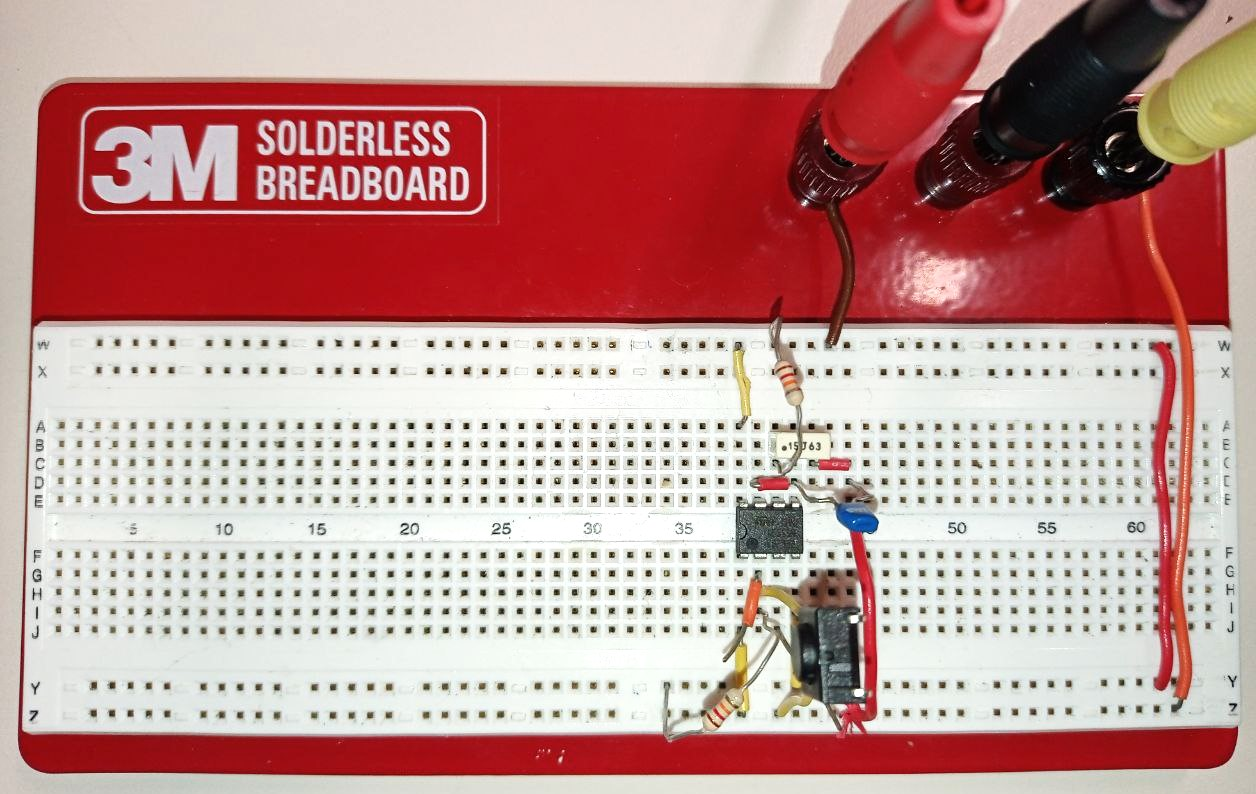
\includegraphics[height=7cm]{immagini/circuito1}
	\caption{Fotografia del circuito monostabile con switch debouncing realizzato in laboratorio.}
	\label{figura:circuito1}
\end{figure}

\noindent Avendo dimensionato in questo modo i componenti, ci si aspetta che la durata dell'impulso in uscita al circuito risulti pari a: \indent$\displaystyle{T = 1.1 \cdot R \cdot C_1 = 1.1 \cdot \SI{12}{\kilo\ohm} \cdot \SI{150}{\nano\farad} = \SI{1.98}{\milli\second}}$
\todo{SBAGLIATO, formula sbagliata? perchè deve risultare > 120 ms}

Dalla figura \ref{figura:TEK00010} è stato verificato che questa durata assumesse un valore maggiore rispetto alla durata dell'impulso in ingresso (che dalla misura effettuata con i cursori dell'oscilloscopio risulta pari a \SI{120}{\milli\second}).

\begin{figure}[h!]
	\centering
	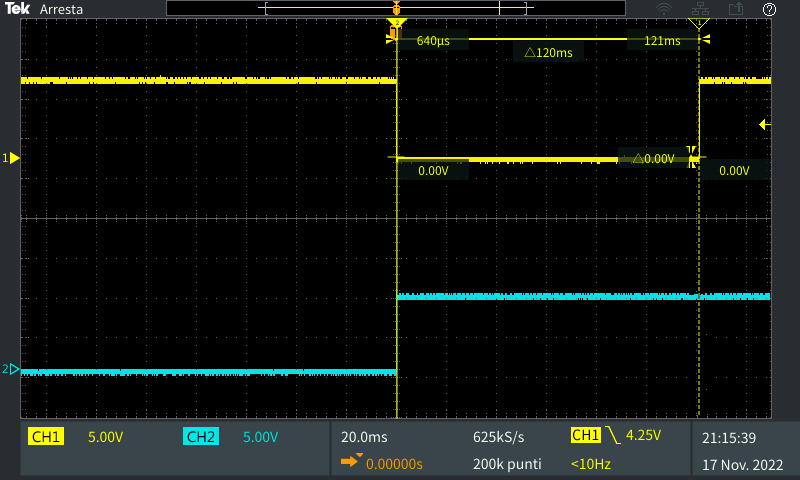
\includegraphics[height=6.5cm]{immagini/TEK00010}
	\caption{Risposta del circuito con cursori.}
	\label{figura:TEK00010}
\end{figure}

\noindent Il segnale ottenuto in uscita è stato riportato nelle figure \ref{figura:TEK00016e17}.

\begin{figure}[h!]
	\centering
	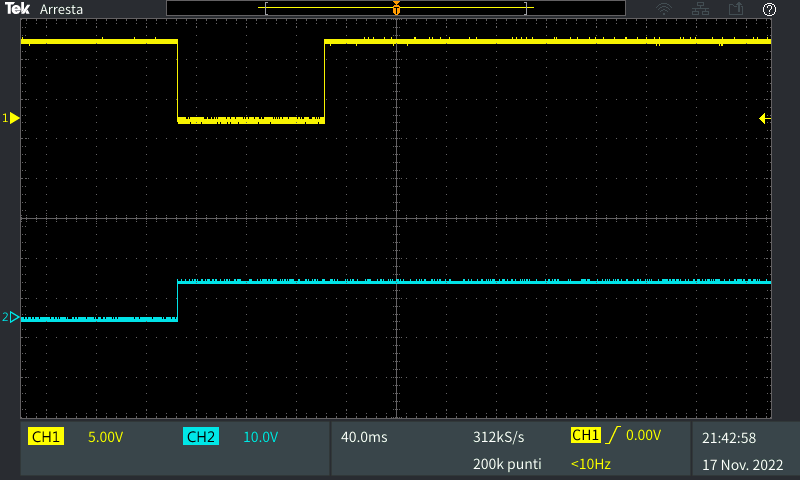
\includegraphics[height=4.6cm]{immagini/TEK00016}
	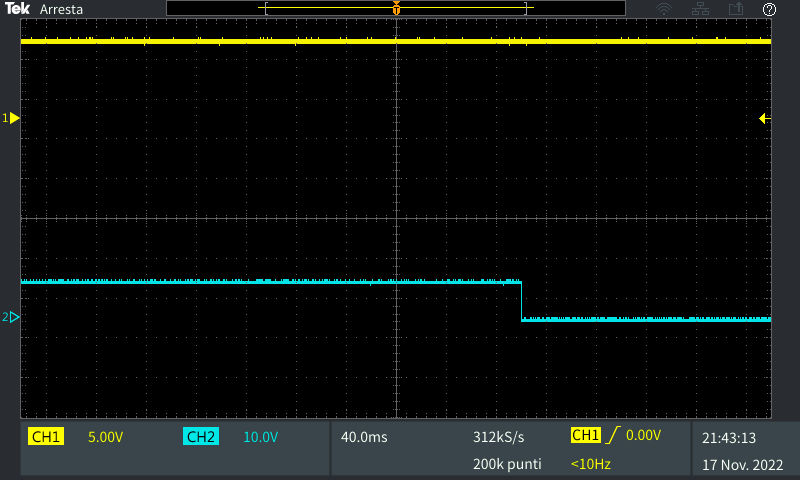
\includegraphics[height=4.6cm]{immagini/TEK00017}
	\caption{Risposta del circuito (ingresso CH1 e uscita CH2).}
	\label{figura:TEK00016e17}
\end{figure}

\noindent Inoltre dalla figura \ref{figura:TEK00009} si vede che il segnale in uscita al LM555 presenta un solo impulso positivo e di conseguenza il timer ha effettivamente corretto il rimbalzo dell'interruttore, di cui è caratterizzato il segnale in ingresso, come preannunciato nella sezione precedente.

\begin{figure}[h!]
	\centering
	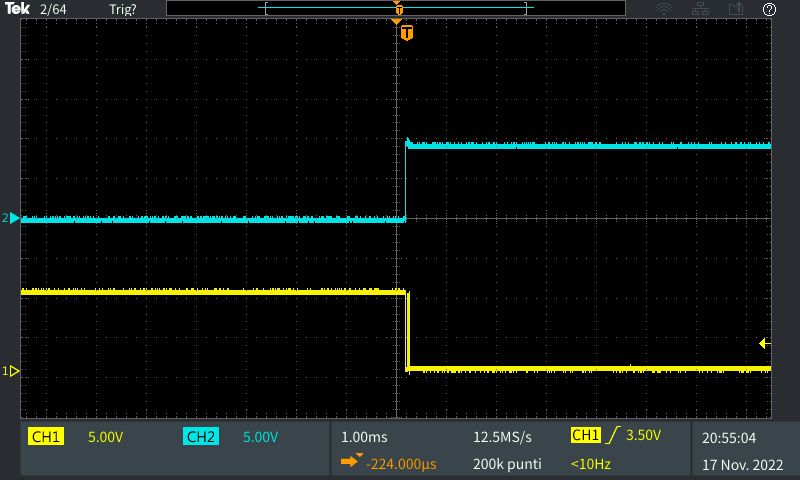
\includegraphics[height=6.5cm]{immagini/TEK00009}
	\caption{Ingrandimento della risposta del circuito (ingresso CH1 e uscita CH2).}
	\label{figura:TEK00009}
\end{figure}

\newpage
\section{Circuito 2: LM555 in configurazione bistabile}\label{sez2}
\subsection{Schema del circuito e Funzione di Trasferimento}
Questo circuito (in figura \ref{figura:schema2}) è costituito da un timer 555, da due resistenze (dette resistenze di pull-up) e da due pulsanti (set e reset).

\begin{figure}[h!]
	\centering
	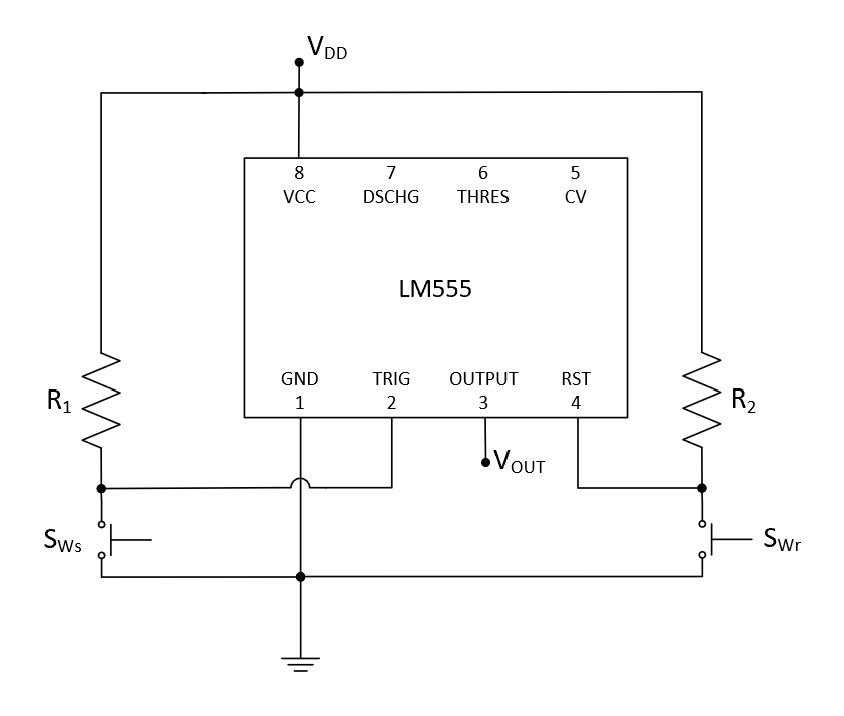
\includegraphics[height=7.5cm]{immagini/schema2}
	\caption{Schema del circuito bistabile.}
	\label{figura:schema2}
\end{figure}

\noindent Si tratta di un circuito bistabile perché presenta due stati stabili, set e reset, che vengono attivati in modo mutuamente esclusivo tramite la pressione di due pulsanti situati tra i rispettivi nodi e la massa. Dunque in ingresso si riceve un segnale che può essere di due tipologie differenti in base all'interruttore attivato: uno per il set oppure uno per il reset che determinano in uscita una transizione al livello logico alto o a quello basso rispettivamente. Perciò la durata dell'impulso positivo presente sul segnale in uscita dipende dal momento in cui il 555 riceve un comando di set e da quello in cui ne riceve uno di reset.

La funzione di trasferimento di questo circuito è:
\begin{equation}
	\begin{cases}
		V_{out}= V_{DD}\indent\indent \mathrm{a\;partire\;dalla\;pressione\;di\;} S_{Ws} \mathrm{\;fino\;alla\;pressione\;di\;} S_{Wr}\\[5pt]
		V_{out}= 0\indent\indent\indent \mathrm{altrimenti}\\
	\end{cases}
\end{equation}

\subsection{Analisi e dati sperimentali}
Per realizzare la breadboard (visibile in figura \ref{figura:circuito2}) sono state utilizzate delle resistenze con un valore di \SI{10}{\kilo\ohm} ciascuna.

\begin{figure}[h!]
	\centering
	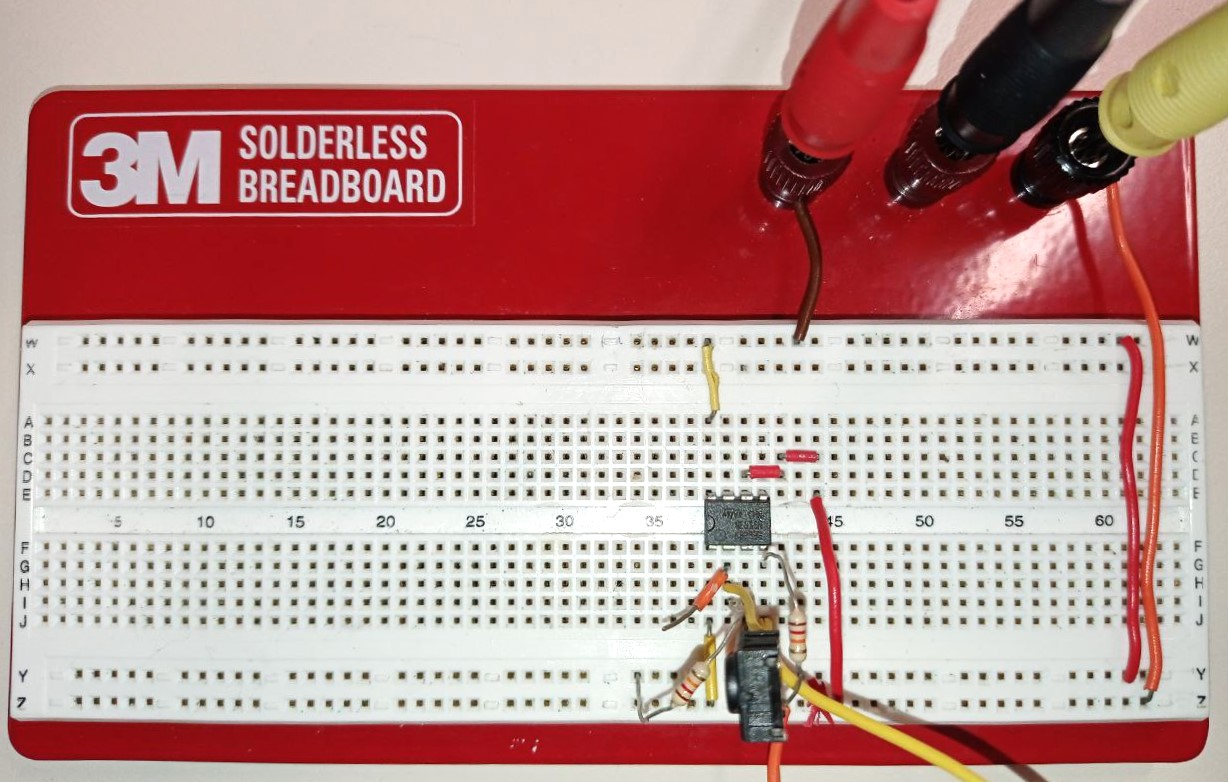
\includegraphics[height=7cm]{immagini/circuito2}
	\caption{Fotografia del circuito bistabile realizzato in laboratorio.}
	\label{figura:circuito2}
\end{figure}

\newpage
\noindent Inizialmente è stato premuto il pulsante di set (mantenendo il pulsante di reset aperto) e questo ha consentito di avere in uscita un segnale al livello logico alto. Successivamente l'attivazione dei due interruttori è stata invertita (disattivando il pulsante di set e attivando quello di reset) ottenendo di conseguenza un segnale in uscita al livello logico basso. Queste variazioni sull'uscita sono state riportate nelle figure \ref{figura:TEK00012e13}.

\begin{figure}[h!]
	\centering
	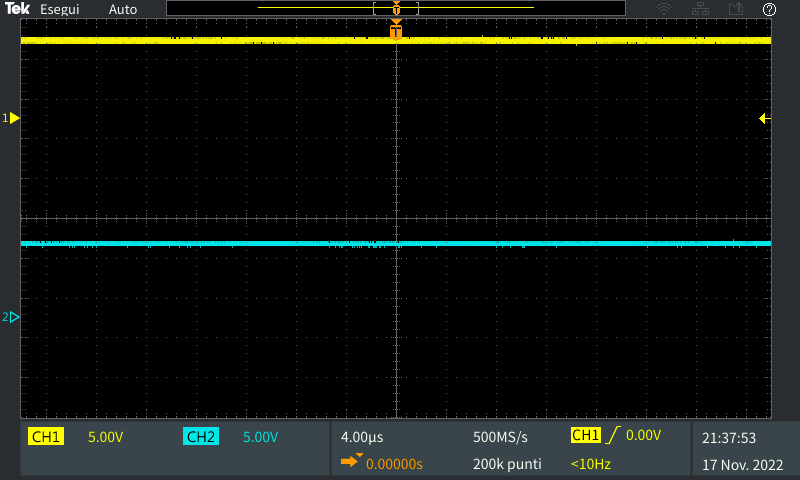
\includegraphics[height=4.6cm]{immagini/TEK00012}
	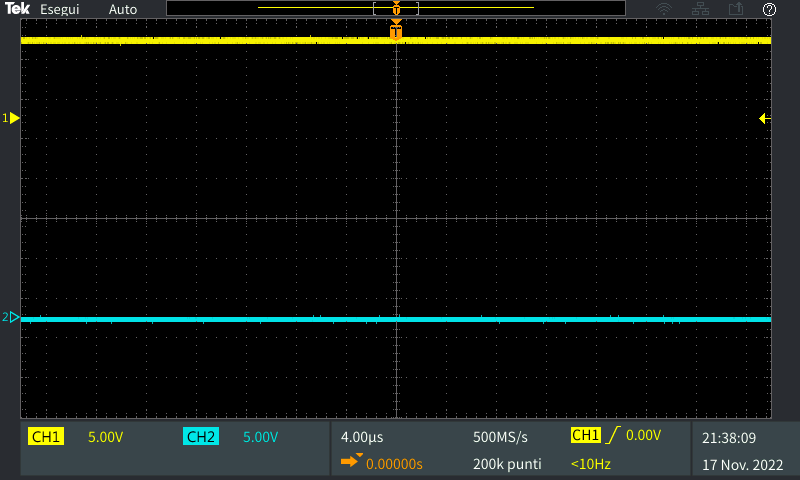
\includegraphics[height=4.6cm]{immagini/TEK00013}
	\caption{Risposta del circuito: a sinistra S ON - R OFF, a destra S OFF - R ON.}
	\label{figura:TEK00012e13}
\end{figure}

\newpage
\section{Circuito 3: LM555 in configurazione astabile}
\subsection{Schema del circuito e Funzione di Trasferimento}
Andiamo ora a studiare l'ultima configurazione del NE555, che è la modalità astabile. Per realizzare il circuito, si utilizzano due capacità e due resistenze: la prima resistenza, $\mathrm{R_A}$, è collegata fra l'alimentazione e il pin 7 del NE555, mentre la seconda, $\mathrm{R_B}$, si trova fra i pin 7 e 2; per quanto riguarda le capacità, $\mathrm{C_1}$ si trova tra il pin 6 e la massa, invece $\mathrm{C_2}$ è connessa tra il pin 5 e la massa. Lo schema si trova in figura \ref{figura:schema3}. \par
In quest'ultima configurazione, il NE555 viene utilizzato per generare un'onda quadra con duty cycle variabile, le cui caratteristiche dipendono dalla rete collegata esternamente al componente. Non abbiamo nessuno stato stabile, l'uscita oscillerà continuamente tra due stati instabili.
\begin{figure}[h!]
	\centering
	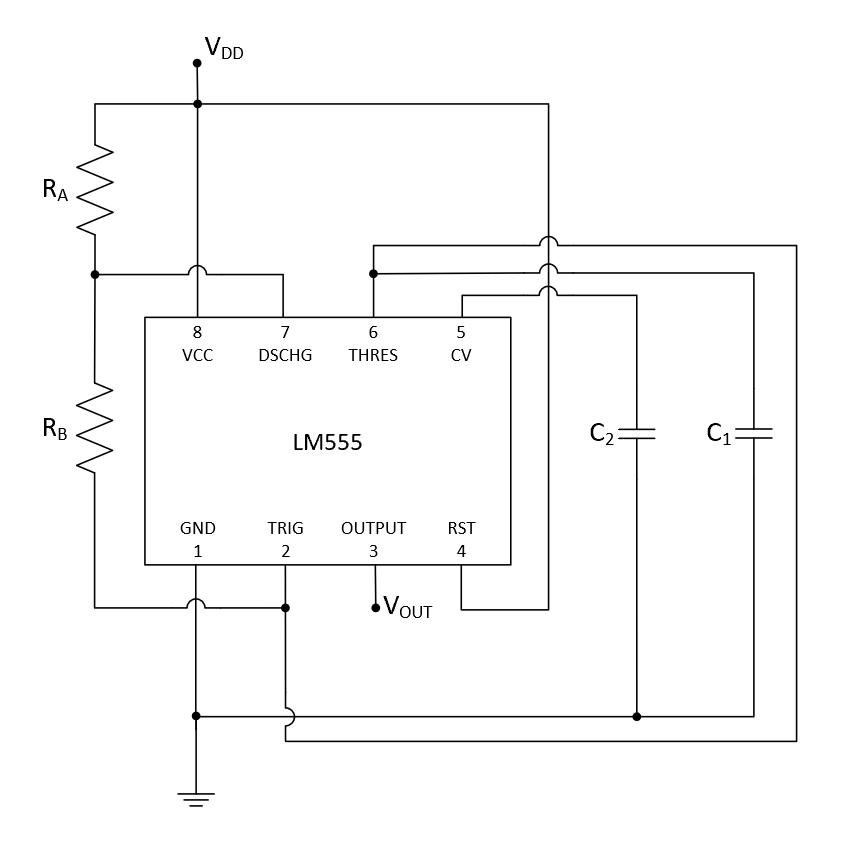
\includegraphics[height=7.5cm]{immagini/schema3}
	\caption{Schema dell'evoluzione del circuito bistabile.}
	\label{figura:schema3}
\end{figure}
\\Il percorso di carica della capacità $\mathrm{C_1}$ avviene attraverso la serie delle resistenze $\mathrm{R_A}$ e $\mathrm{R_B}$, ha inizio quando la tensione ai capi della capacità è di $1/3\cdot V_{DD}$ e termina quando questo valore raggiunge $2/3\cdot V_{DD}$. Durante quest'intervallo, l'uscita va a $\mathrm{V_{DD}}$, quindi rimane alta. Terminata la fase di carica, ha inizio la fase di scarica della capacità $\mathrm{C_1}$ attraverso la resistenza $\mathrm{R_B}$. La scarica continua fin quando la tensione ai capi di $\mathrm{C_1}$ raggiunge il valore di $1/3\cdot V_{DD}$, quindi il ciclo di carica/scarica si ripete. 
% formule + consid dc
\subsection{Analisi e dati sperimentali}
\begin{figure}[h!]
	\centering
	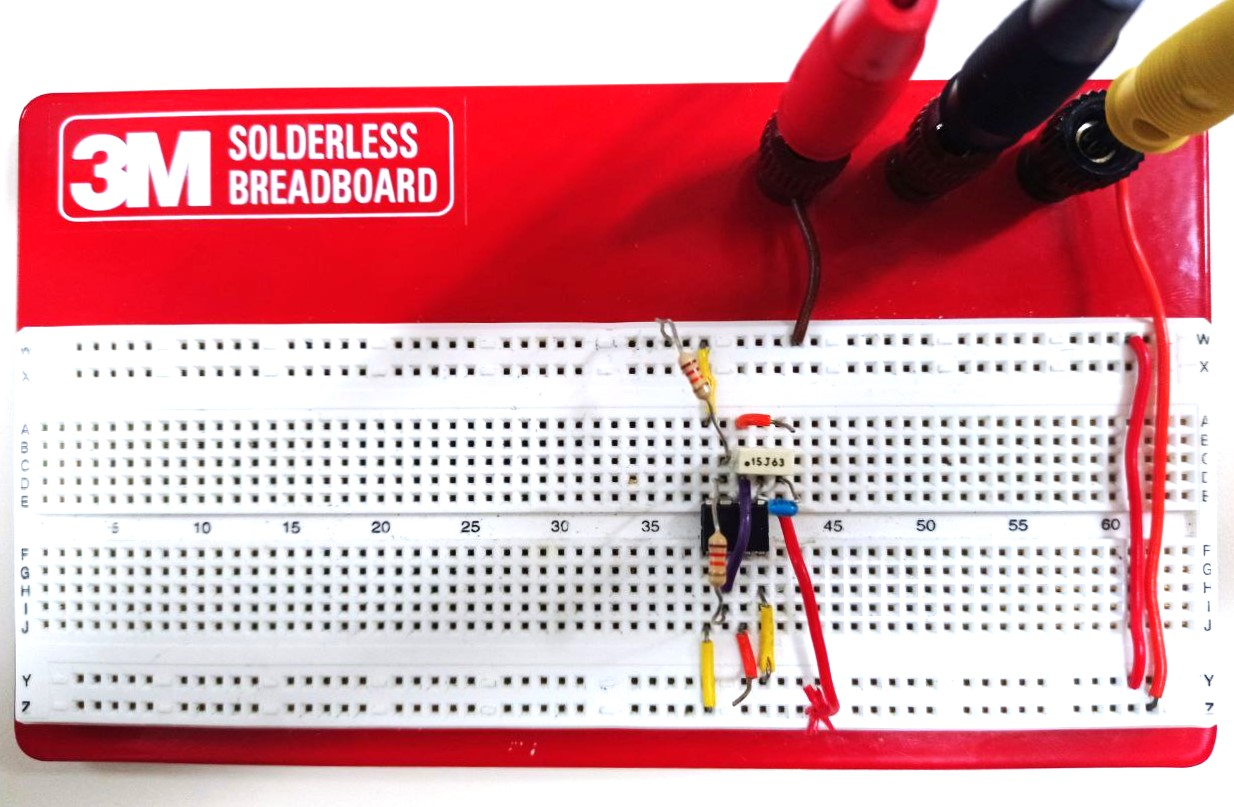
\includegraphics[height=7cm]{immagini/circuito3}
	\caption{Fotografia dell'evoluzione del circuito bistabile realizzata in laboratorio.}
	\label{figura:circuito3}
\end{figure}

\newpage
\section{Circuito 4: Evoluzione del LM555 in configurazione astabile}
\subsection{Schema del circuito e Funzione di Trasferimento}
\begin{figure}[h!]
	\centering
	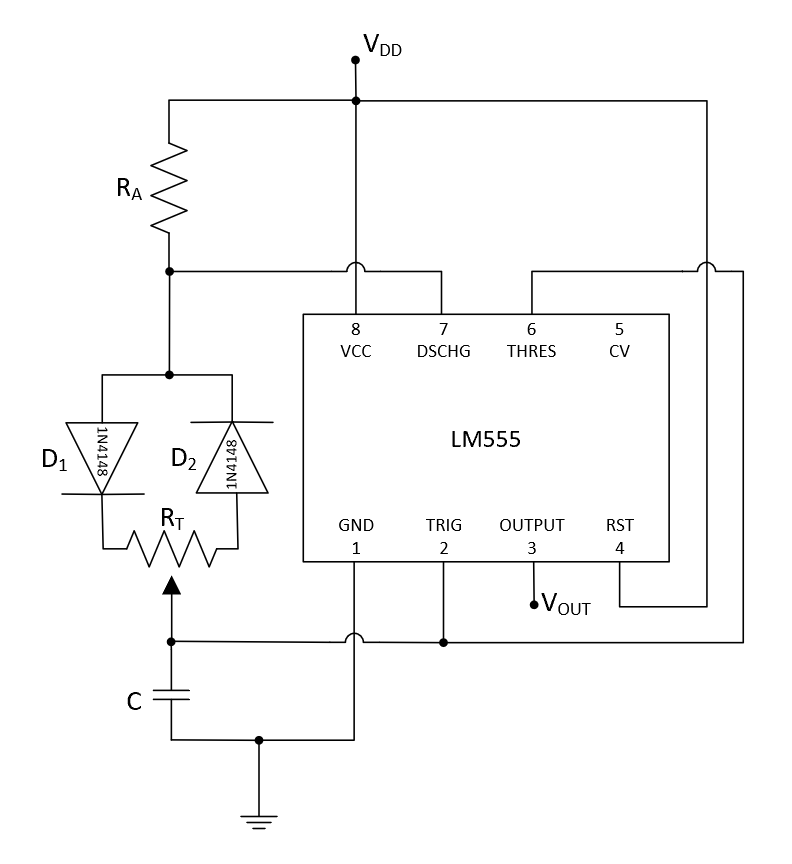
\includegraphics[height=7.5cm]{immagini/schema4}
	\caption{Schema del circuito astabile.}
	\label{figura:schema4}
\end{figure}
\subsection{Analisi e dati sperimentali}
\begin{figure}[h!]
	\centering
	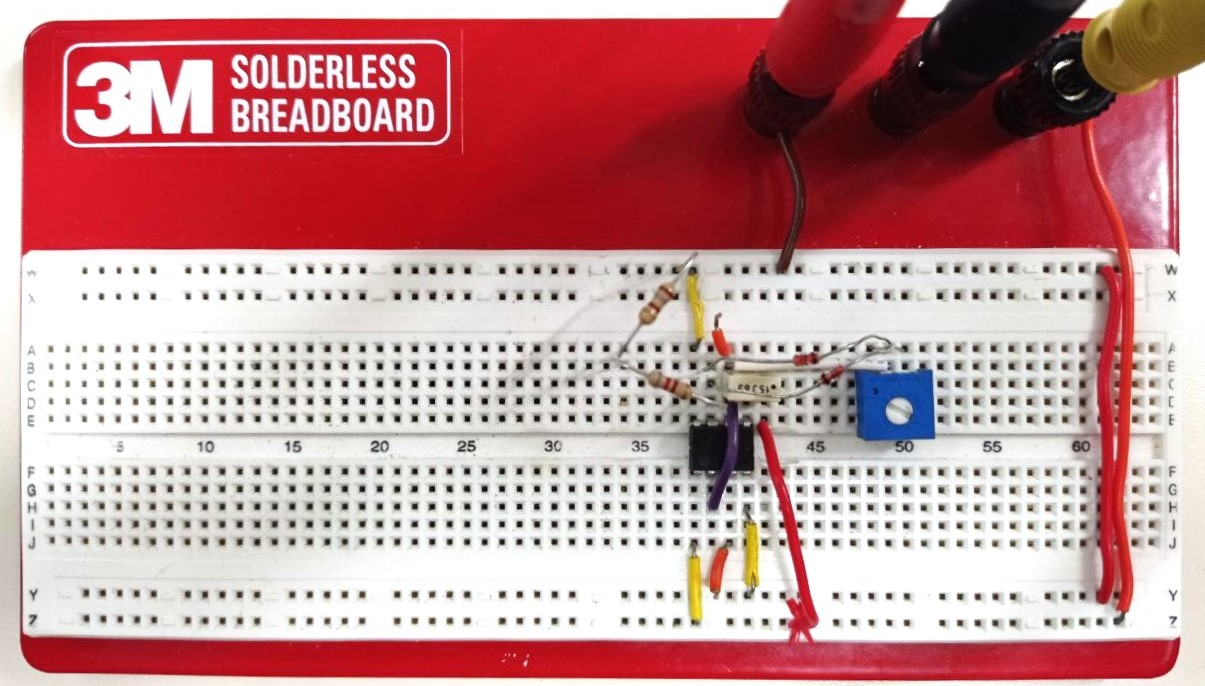
\includegraphics[height=7cm]{immagini/circuito4}
	\caption{Fotografia del circuito astabile realizzato in laboratorio.}
	\label{figura:circuito4}
\end{figure}

%----------------------------------------------------------------------------------------

\end{document}
